\chapter{Testing}
\section{Testing Methodology}

For the testing of the protocol, we implemented a proof-of-concept in Python, using the OpenFHE library\cite{openFHE}. The testing methodology consists of the following steps: firstly, we generate a set of random positions for the parking spots. After that we generated a random position for the client, we computed the z-order encoding for both the client and the parking spots, and finally we computed the distances between the client position and the parking spots using the homomorphic encryption scheme.

\section{Performance Evaluation}

What tested:
\begin{itemize}
    \item Encryption and decryption time for the client position
    \item Distance computation time for the workers
    \item Overall time for the protocol execution
    \item Comparison with clear computation for the client
\end{itemize}

\begin{figure}[h]
    \centering
    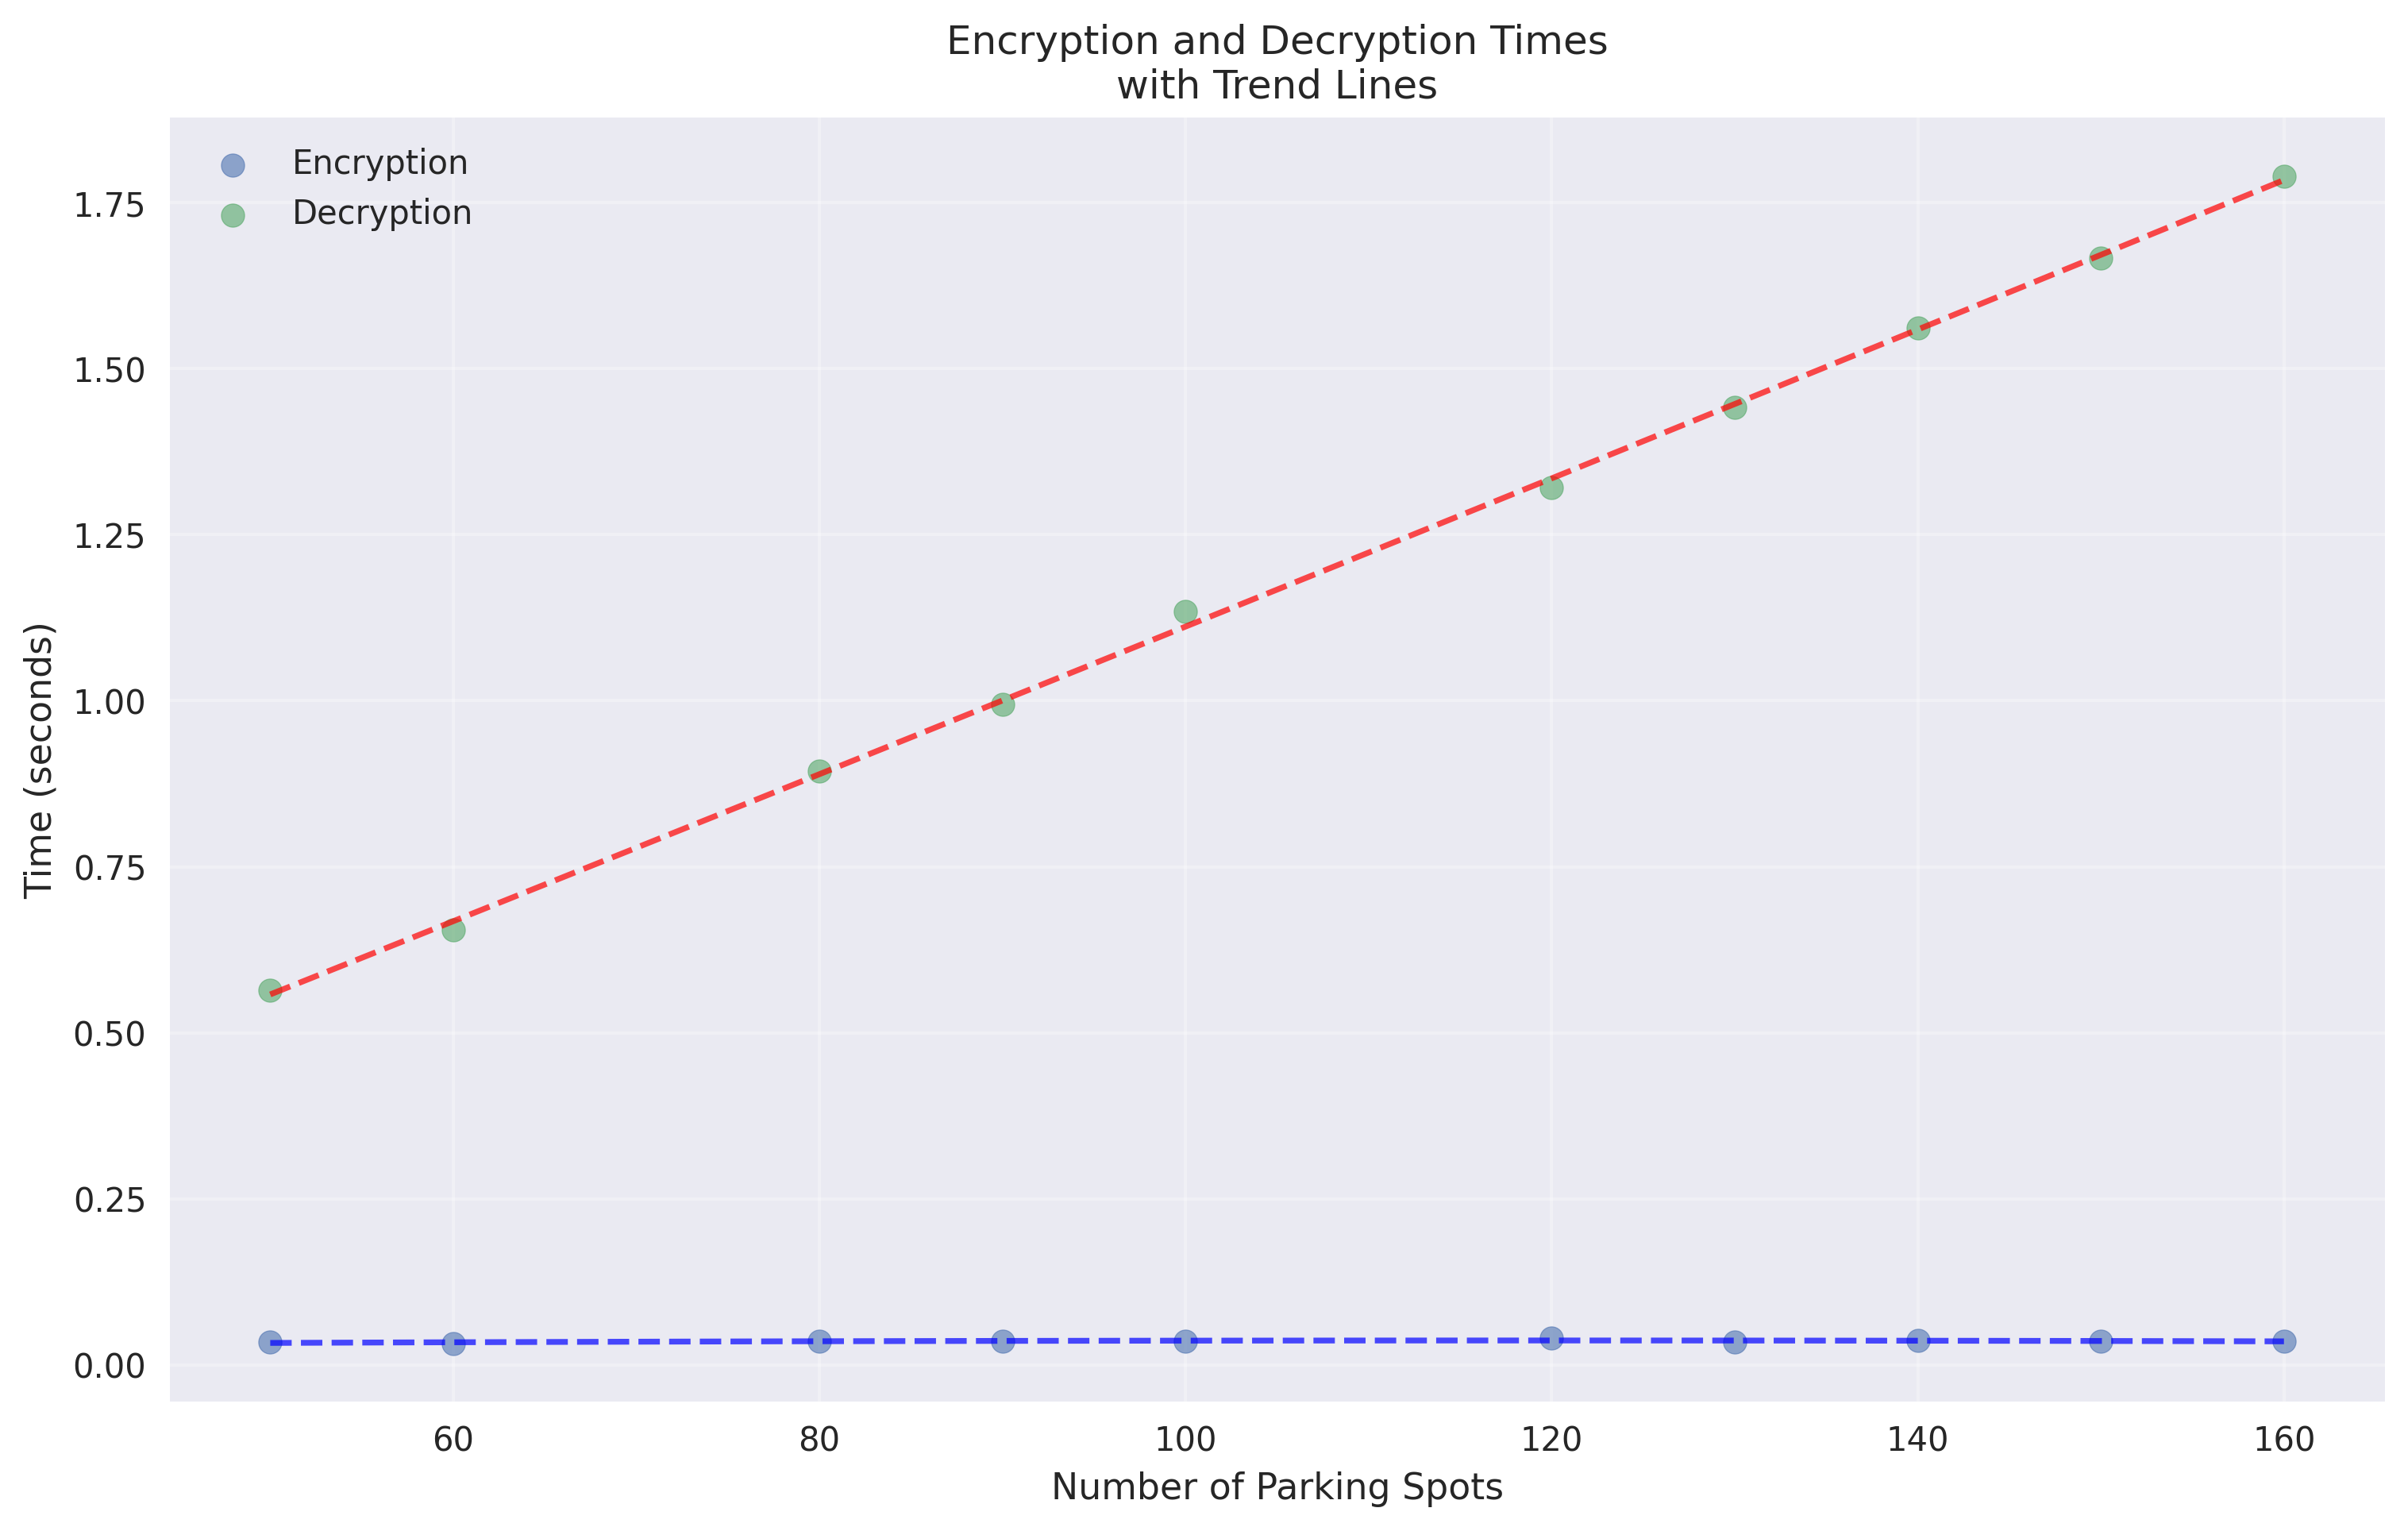
\includegraphics[width=8.5cm,height=7cm]{img/crypto_times.png}
    \caption{Visualization of the Encryption and Decryption time using HE}
    \label{fig:testing}
\end{figure}

\begin{figure}[h]
    \centering
    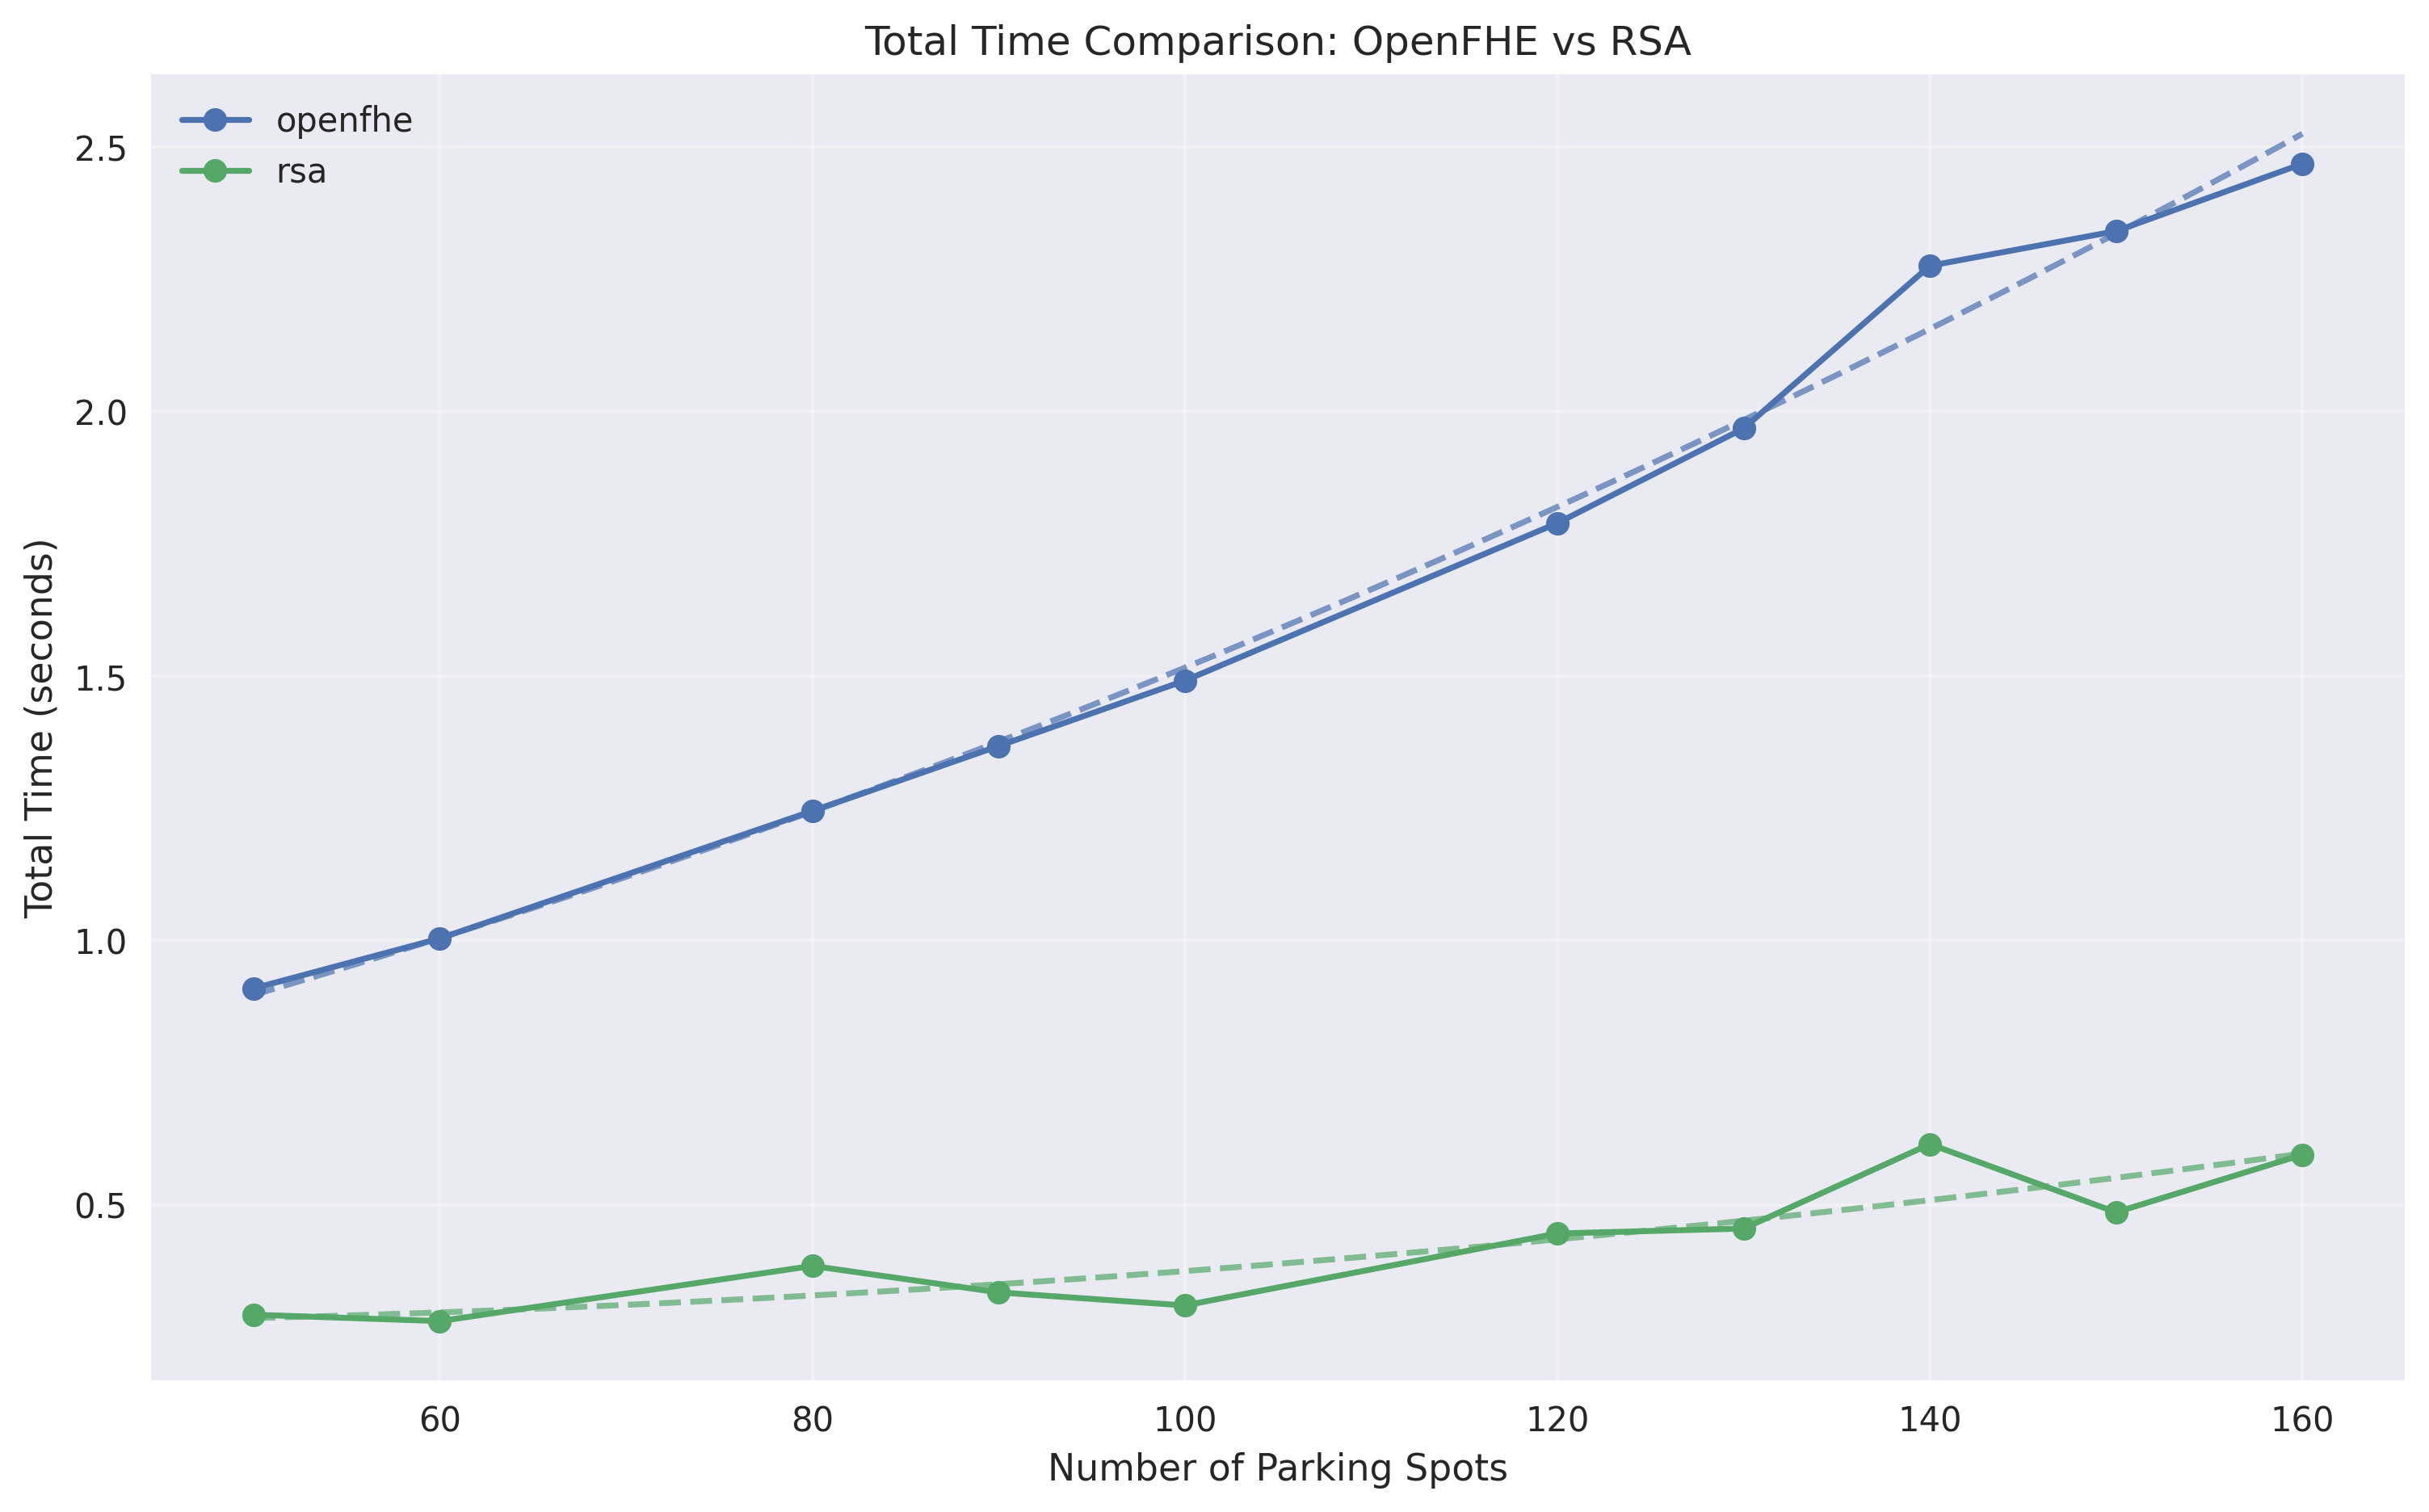
\includegraphics[width=8.5cm,height=7cm]{img/total_time_comparison.png}
    \caption{Comparison between RSA and HE for encryption and decryption}
    \label{fig:he-vs-rsa}
\end{figure}

\section{Security Analysis}

\section{Future Work}
\begin{itemize}
    \item Integrazione della libreria \emph{SEAL Embedded} per i sensori
    \item Definizione della funzione per il calcolo delle distanze
    \item Analisi degli ordini di grandezza degli errori
    \item Selezione delle posizioni rilevanti:
    \begin{itemize}
        \item Area poligonale (due punti)
        \item Area discreta (MGRS)
    \end{itemize}
    \item Deduplicazione di vettori numerici
    \item Ottimizzazione delle richieste per evitare attacchi DoS
    \begin{itemize}
        \item Dimostrazione delle vulnerabilità nell'implementazione precedente
        \item Proposta di patch risolutive
    \end{itemize}
\end{itemize}


\section{Conclusion}

\begin{itemize}
    \item Il test di fattibilità ha dimostrato che l'implementazione del protocollo è possibile e funzionale.
    \item I tempi di esecuzione sono accettabili per un utilizzo in scenari reali.
    \item la sicurezza del protocollo è garantita sotto il threat model considerato
    \item rimane comunque computaziononalmente piu' costoso rispetto ad una soluzione RSA, ma puo' essere applicato ad uno scenario zero trust.
    \item il protocollo è scalabile orizzontalmente in quanto server e sensori ma la CA no.
\end{itemize}
